\documentclass[11pt, oneside]{article} 
\usepackage{geometry}
\geometry{letterpaper} 
\usepackage{graphicx}
	
\usepackage{amssymb}
\usepackage{amsmath}
\usepackage{parskip}
\usepackage{color}
\usepackage{hyperref}

\graphicspath{{/Users/telliott/Github/calculus_book/png/}}
% \begin{center} 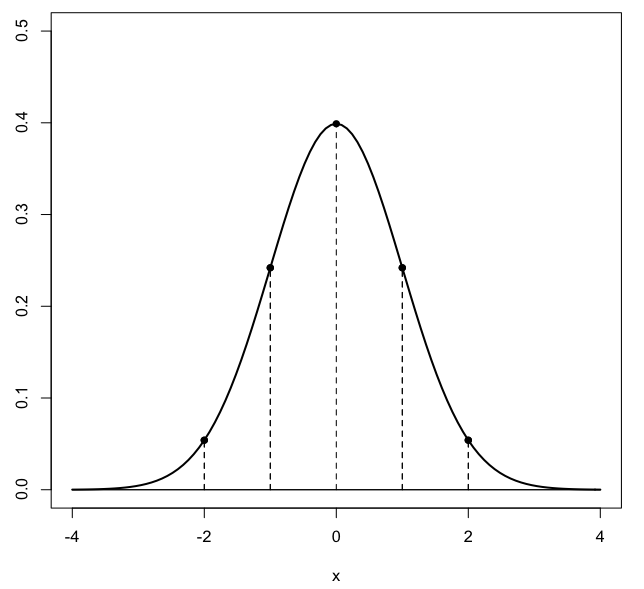
\includegraphics [scale=0.4] {gauss3.png} \end{center}

\title{Pi is a constant}
\date{}

\begin{document}
\maketitle
\Large

\label{sec:Pi_is_a_constant}

\begin{center}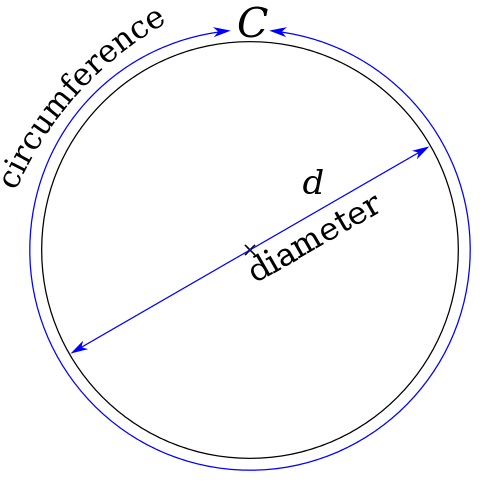
\includegraphics [scale=0.3] {circle0.png}\end{center}

We began the book with a bold claim:  the ratio of the circumference of a circle to its diameter is a constant, independent of the length of the diameter:
\[ \pi = \frac{C}{d} = \frac{C}{2r} \]

We did not prove this theorem at the time but can now.

Proof:

Consider two circles of different sizes on the same center, with inner radius $r$ and outer radius $r'$.

Divide the circles into $n$ equal sectors each with central angle $t$.

Then the arc length $s = C/n$ or $s' = C'/n$.  For any particular $n$ we have that $C/s = C'/s'$.  Thus, it suffices to show that the ratio $s/r = s'/r'$ (i.e. is constant) to prove the theorem.

\begin{center}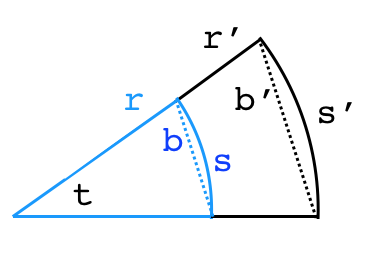
\includegraphics [scale=0.5] {pi9.png}\end{center}
In the limit as $n \rightarrow \infty$, i.e., as the example sector gets smaller and the total number of sectors gets very large, 
$b \approx s$ and $b' \approx s'$.

This is just Archimedes' argument, that as the number of sides of an inscribed regular polygon increases without limit, the perimeter of the polygon will be equal to the circumference of the circle.  Therefore as $n \rightarrow \infty$
\[ s = b; \ \ \ s' = b' \]

But the two triangles are similar, because they share the angle $t$ and are both isosceles.  Therefore, the ratio $b/r$ is equal to the ratio $b'/r'$ and then
\[  \frac{s}{r} = \frac{s'}{r'} \]
so
\[ \frac{C}{r} = \frac{C'}{r'} \]

This completes the proof.

$\square$

Second proof:

Here is a simple variant.  Drop the altitude $h$ in each of the two similar triangles.  The ratio $h/r$ is equal to $\sin t$, but the arc length $s = t$, measured in radians.

\begin{center}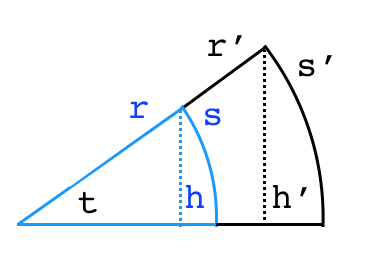
\includegraphics [scale=0.5] {pi10.png}\end{center}

In the limit that $n \rightarrow \infty$, the ratio between $s$ and $h/r$ is equal to our "special limit":
\[ \lim_{n \rightarrow \infty} \ \frac{t}{\sin t} = 1 \]

If the ratio to the sine is equal to $1$, so is the ratio to its inverse and thus the ratio $s/r$ is constant, which is what we wanted to prove.

$\square$

\subsection*{Pi is irrational}

This proof is too challenging for this book.  You can read about it in wikipedia, or

\url{https://mindyourdecisions.com/blog/2013/11/08/proving-pi-is-irrational-a-step-by-step-guide-to-a-simple-proof/}


\end{document}